

\documentclass["../Applied_probabillity _and_statistics_lab_KTU.tex"]{subfiles}
 
\begin{document}
\section{Background Information}
  To be completed. Describe Basic ideas  about probability, distribution function, density, Expectation and  variance.
\section{Simulating Coin Toss}
 The probability of getting a Heads or a Tails on a coin toss is both 0.5.  We can use
R to simulate an experiment of flipping a coin a number of times and compare our results with
the theoretical probability.  

0 = Tails and 1 = Heads


\begin{lstlisting}[language=R]

sample(0:1,15,rep=T)  #flip 15 times
 
# read the manual for sample function and try to under stand the options.
help(sample) 
\end{lstlisting}

Let us write a small function so that we can easily repeat coin toss experiment and calculate probability of getting 1.
 \begin{lstlisting}[language=R]
 flip= function(n) sample(0:1,n,rep=T) # look at the function definition and the argument passing.
 exp1<-flip (100) 	# let us flip 100 times
 prob= sum(exp1==1)/100
 
 exp2= flip(10000);   # a  semi colon suppresses long outputs
 prob= sum(exp2==1)/10000
 
 \end{lstlisting}
 
 Rolling a dice with six faces 20 times can be simulated in R using 
 sample(1:6,20,rep=T).  Write a function to simulate roll of a dice and roll it 10000 time. Compute the probability of getting 4 any number less than 4.
 
 \section{Exploring Probability distributions}
  In this section we will try to explore various probability distributions. R supports many of them. For each distribution for functions are provided pdf cdf  inverse cdf  and a random number generator. 
  The density functions start with d. Eg dnorm() dbinom are densty functions for normal and binomial distributions. The cdf starts with p inverse with q and random number generator with r. Eg rbinom() will give a sample from a binomial distribution.
  
 \section{Normal distribution}
 Gaussian probability distribution is the most important probability distribution we will study.

 
 $P(x) = \frac{1}{{\sigma \sqrt {2\pi } }}e^{{{ - \left( {x - \mu } \right)^2 } \mathord{\left/ {\vphantom {{ - \left( {x - \mu } \right)^2 } {2\sigma ^2 }}} \right. \kern-\nulldelimiterspace} {2\sigma ^2 }}}$
 There are two parameters $\mu$, the mean and $\sigma $ ,the standard deviation.
  Read the documentation of normal distribution.
\begin{lstlisting} [language=R]
help(Normal)
 \end{lstlisting} 
 There are four  function. dnorm pnorm qnorm and rnorm. Let us experiment with each of them. 
 Let us examine dnorm. It give the probability density at a point. For example dnorm(0) will return 0.3989423.
 
 \begin{lstlisting} [language=R]
 x=seq(-10, 10, by = 0.05)      # create  a vector of numbers between -10 ad 10
 y=dnorm(x)                     # find probability density at each point in the above vector
 plot(x,y)                      #plot 
 
 \end{lstlisting}
 
 Your out put will look like figure 1
\begin{figure}
 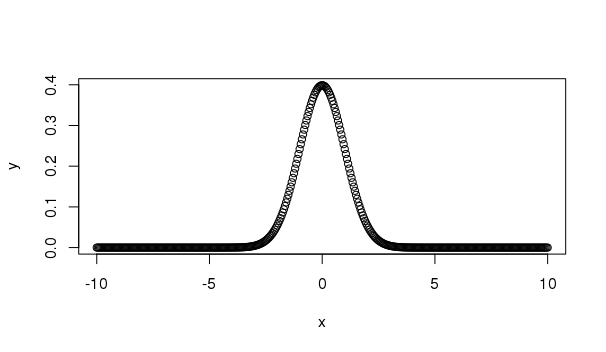
\includegraphics[scale=.4]{images/normal.png}
 \label{norm}
 \end{figure} 
 
 The above code assumes that you are using a normal distribution of mean=1 and sd=1. You can change both parameters.
 
 \begin{lstlisting} [language=R]
 dnorm(0,mean=4,sd=10)  # density at 0 from a distribution with mena 4 and sd=10
 \end{lstlisting}

Try plotting the distribution for different values of mean and standard deviation. Observer how the curve looks like.

Pnorm function give the cumulative   distribution. 
 \begin{lstlisting} [language=R]
  pnorm(0)   #cdf at 0
  
  #plot cdf  from -10 to 10 
   x <- seq(-20,20,by=.1)
   plot(pnorm(x))

 \end{lstlisting}

\begin{figure}
 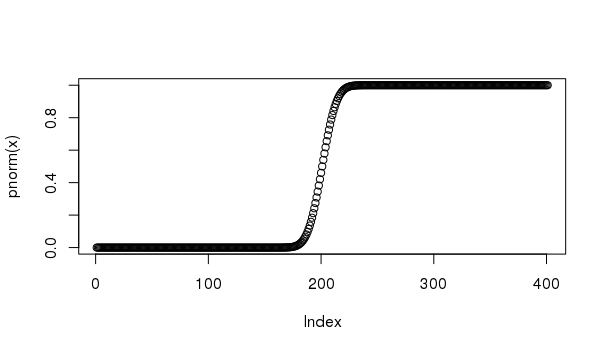
\includegraphics[scale=.4]{images/normal_cdf.png}
 \label{norm}
 \end{figure} 
Here also you can change mean and standard deviation. If you wish to find the probability that a number is larger than the given number you can use the lower.tail option. eg.  pnorm(0,mean=2,lower.tail=FALSE)

The next function we look at is qnorm which is the inverse of pnorm. The idea behind qnorm is that you give it a probability, and it returns the number whose cumulative distribution matches the probability. 
%For example, if you have a normally distributed random variable with mean zero and standard deviation one, then %if you give the function a probability it returns the associated Z-score:
% MORE explantion needed.

\begin{lstlisting} [language=R]
 x <- seq(0,1,by=.05)
 y <- qnorm(x)
   plot(x,y
\end{lstlisting}

The last function rnorm returns a  random number whose probability distribution is normal.
\begin{lstlisting} [language=R]
  rnorm(4)  # generate 4  random nos. from normal distribution.
  rnorm(4,mean=3,sd=3)  # generate 4  random nos. from normal distribution with mean 3 and sd 3
\end{lstlisting}
Let us examine the histogram of a series of random numbers picked from a normal distribution.


\begin{lstlisting} [language=R]
  y=rnorm(2000)  # generate 2000  random nos. from normal distribution.
  hist(y)
\end{lstlisting}

Try increasing the  size of y above and observe how the histogram tends to a normal distribution.

\section{Binomial Distribution}

Read the documentation of binomial distribution.

\begin{lstlisting} [language=R]
help(Binomial)
\end{lstlisting}

The binomial distribution requires two extra parameters, the number of trials and the probability of success for a single trial. The commands follow the same kind of naming convention, and the names of the commands are dbinom, pbinom, qbinom, and rbinom.
\begin{lstlisting} [language=R]
  x <- seq(0,50,by=1)
  y <- dbinom(x,50,0.2) # 50 trials with probability of success 0.2
  plot(x,y)
  y <- dbinom(x,50,0.6)
  plot(x,y)
  x <- seq(0,100,by=1)
  y <- dbinom(x,100,0.6)
  plot(x,y)
\end{lstlisting}

\section{Poisson distribution}
Read the documentation of Poisson distribution

\begin{lstlisting} [language=R]
help("Poisson")
\end{lstlisting}


\begin{lstlisting} [language=R]
 dpois()   to be completed as above
\end{lstlisting}
\end{document}